\chapter{An Approach to Resource-centric Organizational Modeling}
\label{chap:approach}

This section describes about the technical approach that have been taken to solve the problem mentioned in problem statement section of Chapter \ref{chap:introduction}. This chapter also provides an outline of the design, the methodology and overall structure of the approach. The first section of this chapter provides an overview of modeling process approach. The second section compares and evaluates the approach to the existing approaches. The third section discusses the design methodology followed to realise this approach of developing a descriptive modeling web based editor. It also provides a brief description about the frameworks and libraries used. The third section discusses in detail about the \textit{top-down approach}, which has been used to realise the resource-centric organizational modeling. The final section discusses in detail about the relationship between each entity types of this approach. 

%%%%%%%%%%%%%%%%%%%%%%%%%%%%%%%%%%%%%%%%%%%%%%%%%%%%%%%%%%%%%%%%%%%%%%%%%
\section{Overview of Modeling Process}
\label{sec:overviewmodelingprocess}
%%%%%%%%%%%%%%%%%%%%%%%%%%%%%%%%%%%%%%%%%%%%%%%%%%%%%%%%%%%%%%%%%%%%%%%%%
The main focus of this approach is to develop a editor which can be used by business experts to model the informal processe. AS we mentioned before the input, the resource definitions required for the editor is made available from the first phase P1 of the InProXec approach. The resource models provided from this phase is of interrelated in type, which has been explained in detail in the following Section \ref{sec:capIntRel}. The business experts develop informal process models through the editor using these resources to achieve main intention that contains sub-intentions, strategies etc. The reason for designing Informal Processes as models, because these models specify informal processes and provides means of execution for the phases P3 and P4 of InProXec.  

The model provides necessary concepts and relations for modeling the core elements of resource centric organizational modeling. Resources are abstract description which are made concrete during initialization of an instance. There are also resource specific views based on the participating resources' role. 

  


Initializing resource-centric informal process models requires \textit{acquiring} and engaging interrelated resources.

%%%%%%%%%%%%%%%%%%%%%%%%%%%%%%%%%%%%%%%%%%%%%%%%%%%%%%%%%%%%%%%%%%%%%%%%%
\section{Design Methodology}
\label{sec:designmethodology}
%%%%%%%%%%%%%%%%%%%%%%%%%%%%%%%%%%%%%%%%%%%%%%%%%%%%%%%%%%%%%%%%%%%%%%%%%

On the left list we should have all organizational context definitions and on the right one only ones that are contained in an informal process. The dropdown box of the initial and final context defines the selection inside of an informal process, thus right side.

So, in db.cljs, we should have only a list of context definitions no :initial-contexts and :desired-final-contexts. Only :organizational-contexts and under this all available contexts. Under the left list, we present these elements. Right list should refer to the initial-context, final-contexts, etc. of the informal process model depending on the selection of the dropbox button. For instance if we have initial contexts selected on the dropdown box, we should present the initial contexts in the right list.

I have changed the code accordingly and provided you an example how you should change data from views.cljs. All data should be stored in db.cljs. This applies to the text fields of all elements. Whenever, we want to update something we need to update the map in db.cljs and this will be propagated to the views.


On the left side of each list item, you should present all available items of context definitions or intentions whatever type is selected there. On the right side only the ones contained in the respective informal process model. Inside of another entity, you should refer to other entities using their ids and these ids should be resolved using, for instance, intentions vector. You check each intention in the intentions vector, if it’s id is the same as the id you are looking for it, you found it and you use the information about it.  


Please align it with the structure and names of the IPSM.xsd. Each variableName like this is written like variable-name. Each complex type is a map each attribute is a key value pair and each element in another element is another key value pair.


%%%%%%%%%%%%%%%%%%%%%%%%%%%%%%%%%%%%%%%%%%%%%%%%%%%%%%%%%%%%%%%%%%%%%%%%%
\subsection{Specifications}
\label{subsec:specifications}
%%%%%%%%%%%%%%%%%%%%%%%%%%%%%%%%%%%%%%%%%%%%%%%%%%%%%%%%%%%%%%%%%%%%%%%%%
In order to realize the web editor of Intention-centric Organizational Modeling, a formal inquiry has been done and concluded with the below specifications.

\begin{enumerate}   
	\item \textbf{Clojurescript} as the programming language
	\item \textbf{IntelliJIDEA} as the IDE
	\item \textbf{MVC} as the architecture pattern
	\item \textbf{Re-frame} as the pattern for writing SPAs in ClojureScript, using Reagent	
\end{enumerate}

%%%%%%%%%%%%%%%%%%%%%%%%%%%%%%%%%%%%%%%%%%%%%%%%%%%%%%%%%%%%%%%%%%%%%%%%%
\subsection{MVC Architecture}
\label{subsec:mvcarch}
%%%%%%%%%%%%%%%%%%%%%%%%%%%%%%%%%%%%%%%%%%%%%%%%%%%%%%%%%%%%%%%%%%%%%%%%%
 The architecture of the UI editor is based on the \textbf{Model-View-Control (MVC)} design pattern. The MVC paradigm allows to separate business logic from the code that controls presentation and event handling \cite{Oracle2016}.Each entity view in the web page is made up of combination of at least on Model and View, and one or more Controls. The individual files which acts an Model, View and Controller has been shown in the Figure \ref{fig:mvc_arch}

\begin{itemize}
	\item \textbf{Model} artifact stores the required data structure for web-editor. In the developed model artifact, the four main types of data stored inside the artifact are intentions, strategies, capabilities and informal process instances. 
	\item \textbf{View} artifact contains HTML elements and HTML constructs that describe the way of displaying the data from Model to the user.
	\item \textbf{Control} artifact contains the handler functions which can only change the model. Even the initial values of the model are put inside the control. 
\end{itemize}


\begin{figure}
	\centering
	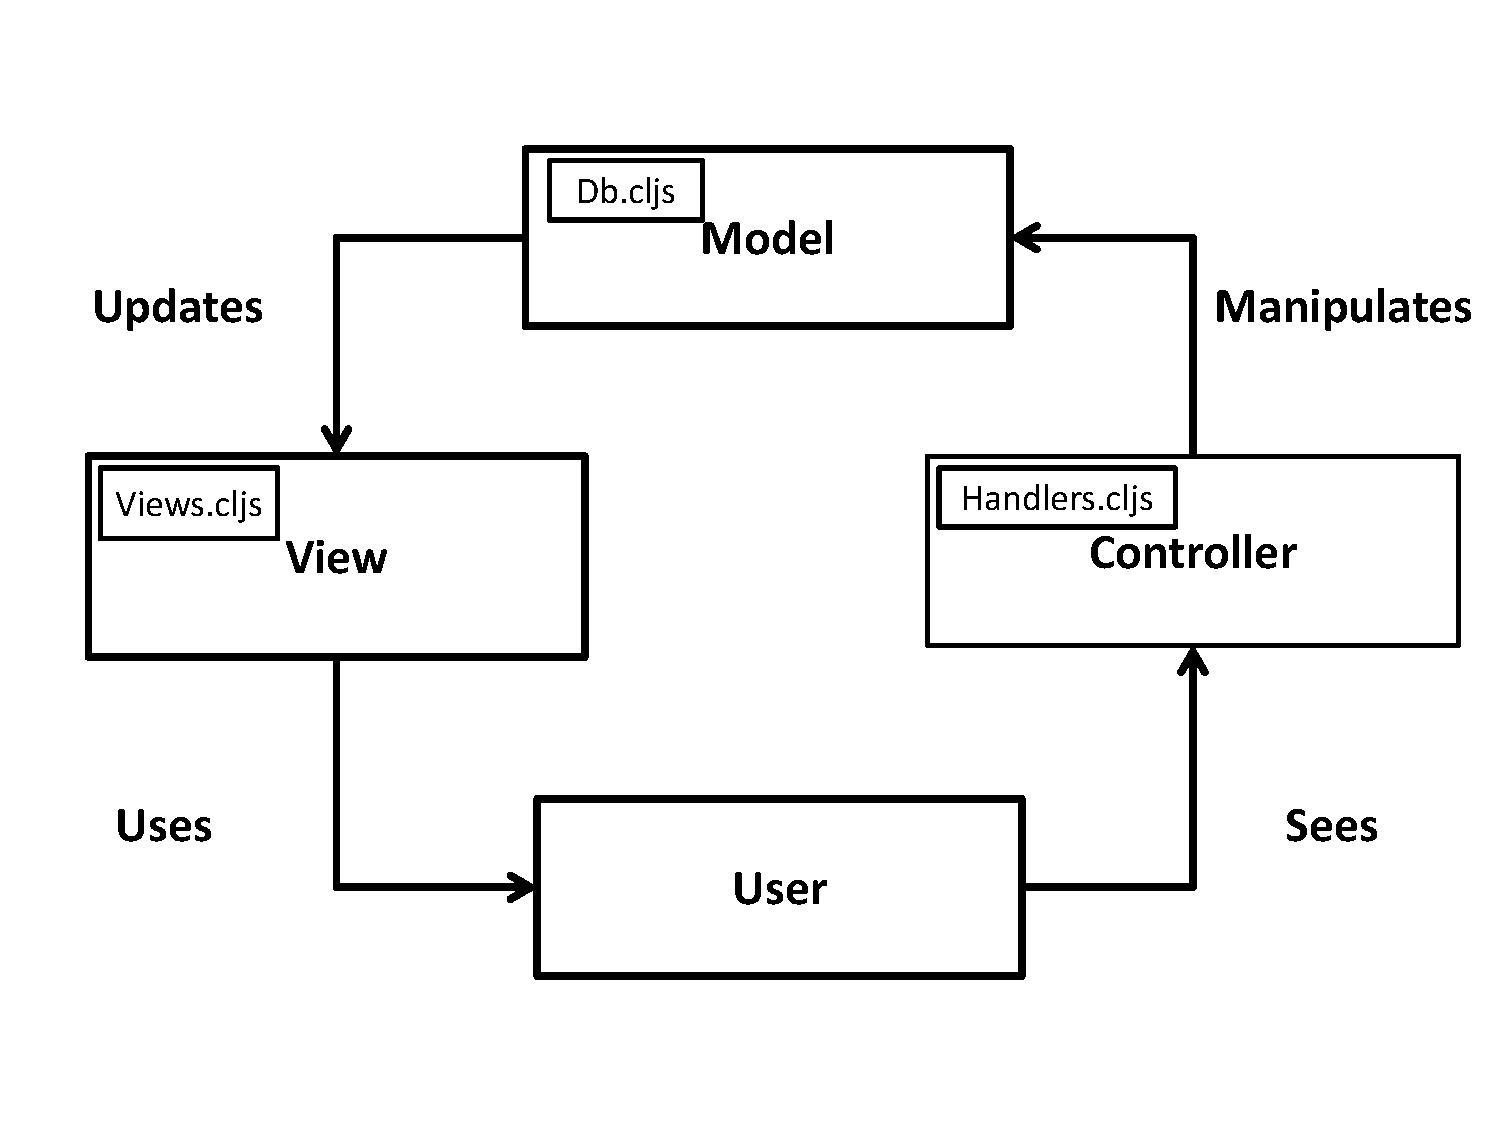
\includegraphics [width= 0.75\textwidth]{mvc_arch.pdf}
	\caption{Relationship between developed web editor artifacts and MVC architecture components}
	\label{fig:mvc_arch}
\end{figure}


%%%%%%%%%%%%%%%%%%%%%%%%%%%%%%%%%%%%%%%%%%%%%%%%%%%%%%%%%%%%%%%%%%%%%%%%%
\subsubsection{Example: Component using MVC Pattern }
%%%%%%%%%%%%%%%%%%%%%%%%%%%%%%%%%%%%%%%%%%%%%%%%%%%%%%%%%%%%%%%%%%%%%%%%%
 The Figure \ref{fig:mvc_arch} below shows the simplifed version of how the components interact with each other using the Model-View-Control (MVC) pattern, for the functionality adding new entity data. This functionality is same for all the types intentions, strategies, capabilities and informal proceess instances and below is the detailed explanation of each interaction.

\begin{enumerate}
	\item User clicks the tab \textbf{Add New} in the web editor.
	\item View, in response to the user click displays the UI component for entering the new entity data details.
	\item User enters the required basic details for adding new entity data and clicks save button.
	\item View dispatches the data to Control, which can only modify the Model.
	\item Control inserts/updates data into the model.
	\item View displays the updated model as it has been subscribed to the model.
\end{enumerate}

\begin{figure}
	\centering
	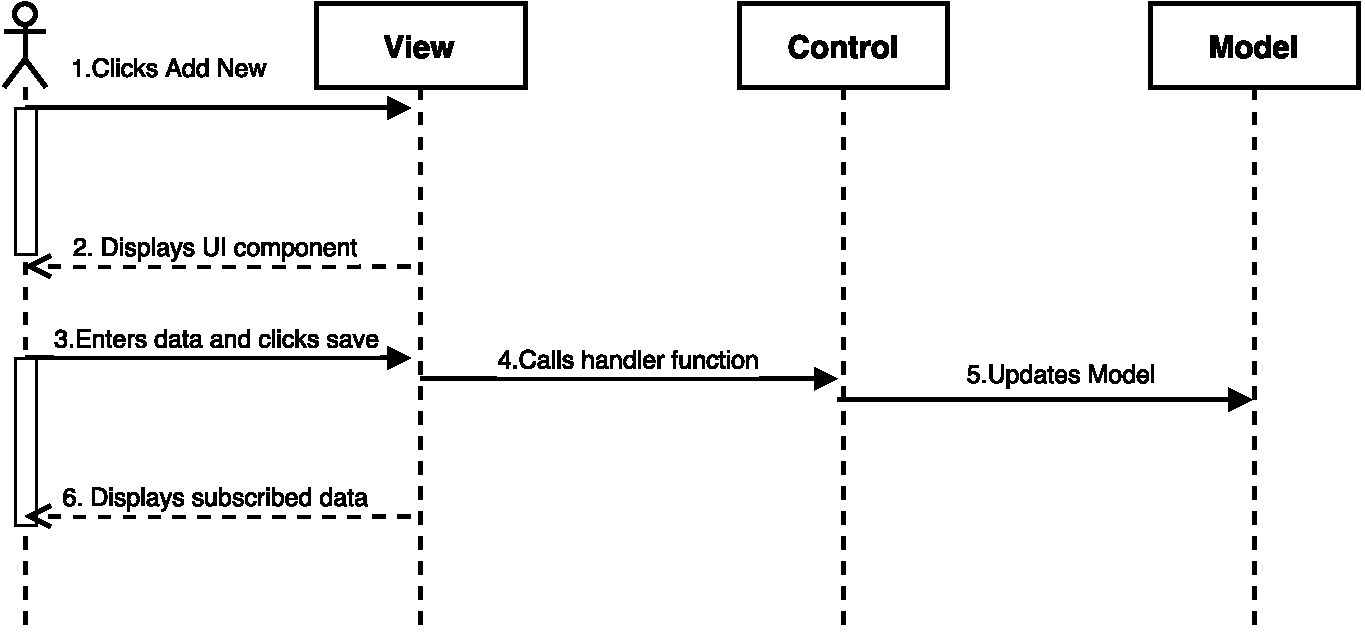
\includegraphics [width= \textwidth]{mvc_pattern.pdf}
	\caption{MVC Pattern of adding new entity}
	\label{fig:mvc_pattern}
\end{figure}


%%%%%%%%%%%%%%%%%%%%%%%%%%%%%%%%%%%%%%%%%%%%%%%%%%%%%%%%%%%%%%%%%%%%%%%%%
\subsection{Using Reagent Framework}
\label{subsec:reagent}
%%%%%%%%%%%%%%%%%%%%%%%%%%%%%%%%%%%%%%%%%%%%%%%%%%%%%%%%%%%%%%%%%%%%%%%%%

The Reagent Framework architecture has been reused Fig. \ref{fig:mvc_pattern23} \footnote{Source: https://github.com/Day8/re-frame}






%%%%%%%%%%%%%%%%%%%%%%%%%%%%%%%%%%%%%%%%%%%%%%%%%%%%%%%%%%%%%%%%%%%%%%%%%
\section{A Top-Down Modeling Approach}
\label{sec:topdownapproach}
%%%%%%%%%%%%%%%%%%%%%%%%%%%%%%%%%%%%%%%%%%%%%%%%%%%%%%%%%%%%%%%%%%%%%%%%%
Intentions are defined hierarchically, intentions can contain and extend intentions which are called as sub-intentions. Intentions can contradict to itself as well. Intentions are associated with strategies, thus intentions can be realized through strategies. Strategies are associated with capabilities. These capabilities are of two types \textit{functional capabilities} and \textit{cross functional capabilities}. Functional capabilities are associated with resources and cross functional capabilities are associated with functional capabilities. Each informal process model is a strategy that has capabilities, strategies, resources that are created out of capabilities and intentions. 

\begin{figure}
	\centering
	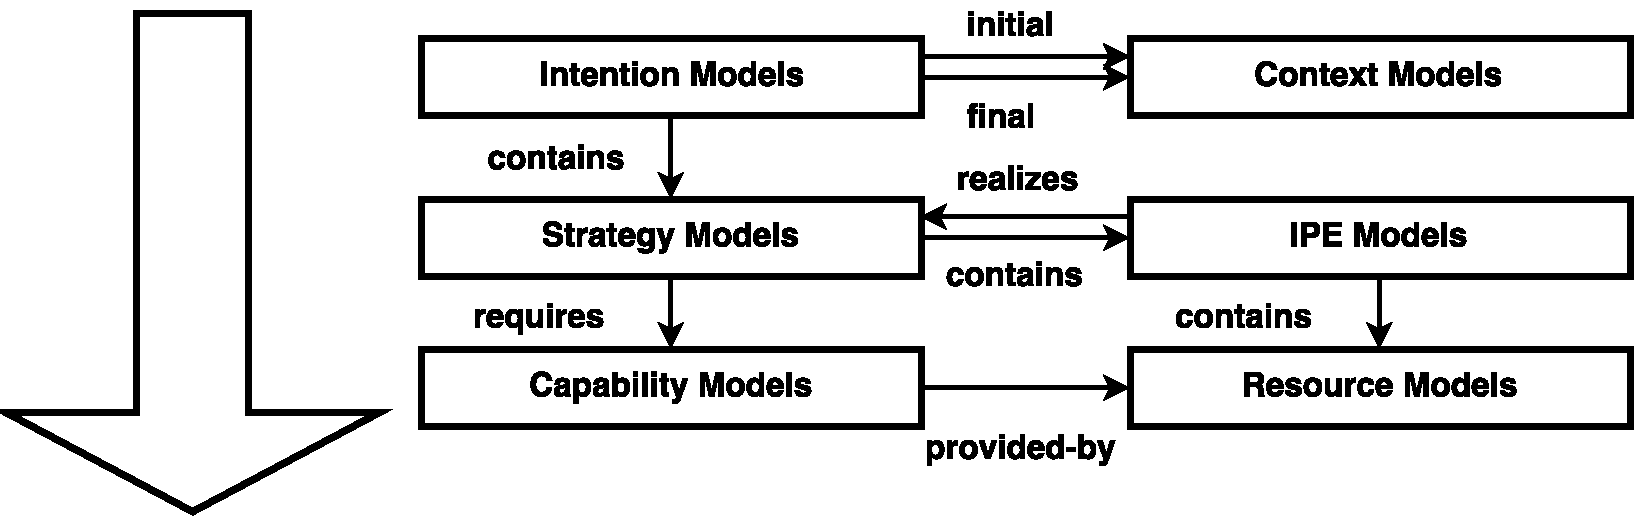
\includegraphics[width=\textwidth]{TopDownApproach.pdf}
	\caption{Top Down Modeling Approach}
	\label{fig:topdownapproach}
\end{figure}

Bider et al \cite{bider2005strategy} propose a strategy-driven modeling approach of processes. Processes are defined based on the goals and refinement continues until meaningful operation level is reached. Consequently, created models are easily changeable as they are decoupled from their operational terms. Such declarative approaches provide more flexibility and enable easier change of the business process models \cite{Sungur2016}.  

%%%%%%%%%%%%%%%%%%%%%%%%%%%%%%%%%%%%%%%%%%%%%%%%%%%%%%%%%%%%%%%%%%%%%%%%%
\section{Characteristics of the Entity Types}
\label{sec:enttyperelation}
%%%%%%%%%%%%%%%%%%%%%%%%%%%%%%%%%%%%%%%%%%%%%%%%%%%%%%%%%%%%%%%%%%%%%%%%%
The entity types are modeled as descriptive informations, this is because models can be initialized and can be made runnable elements which are required in phases P3 and P4 of InProXec. An IPE model describes the main intention that reflects the informal process' main goal. Each intention may be refined into sub-intentions. The IPE model's initial context specified the triggers that signal when model's corresponding resources should be initialized and subsequently work towards the informal process' main intention\cite{Sungur2015a}. The final context specifies conditions for determining the processes' main intention as successfully achieved. 



%%%%%%%%%%%%%%%%%%%%%%%%%%%%%%%%%%%%%%%%%%%%%%%%%%%%%%%%%%%%%%%%%%%%%%%%%
\subsection{Context Intention Relationship}
\label{sec:ctxintrel}
%%%%%%%%%%%%%%%%%%%%%%%%%%%%%%%%%%%%%%%%%%%%%%%%%%%%%%%%%%%%%%%%%%%%%%%%%
Intentions connect initial context definitions with final context definitions Figure \footnote{C Timurhan Sungur, An approach to supporting and automating informal processes, May 2015}.


\begin{figure}
	\centering
	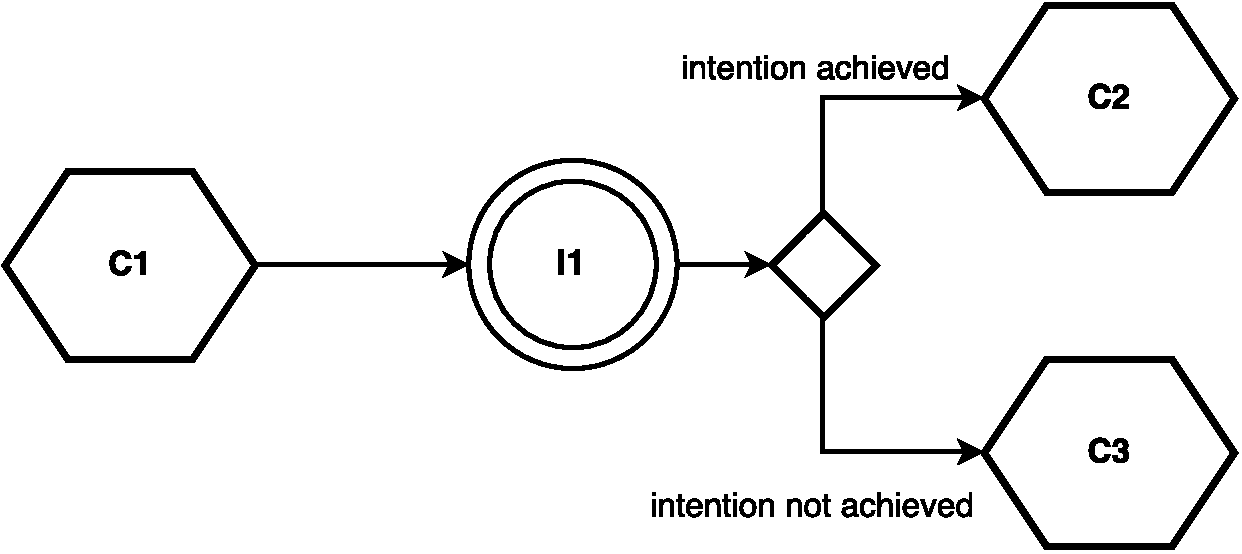
\includegraphics[width=\textwidth,angle=0]{orgIntContext.pdf}
	\caption{Context Intention Relationship}
	\label{fig:orgIntentions}
\end{figure}

%%%%%%%%%%%%%%%%%%%%%%%%%%%%%%%%%%%%%%%%%%%%%%%%%%%%%%%%%%%%%%%%%%%%%%%%%
\subsection{Capabilities Resource Relationship}
\label{sec:capIntRel}
%%%%%%%%%%%%%%%%%%%%%%%%%%%%%%%%%%%%%%%%%%%%%%%%%%%%%%%%%%%%%%%%%%%%%%%%%
Each organizational capability must be provided by a resource in the organization. Resource models are optional to make precise definitions of resources needed. The relationship between organizational capabilities and organizational intentions has been provided in the Figure 
 
\begin{figure}
	\centering
	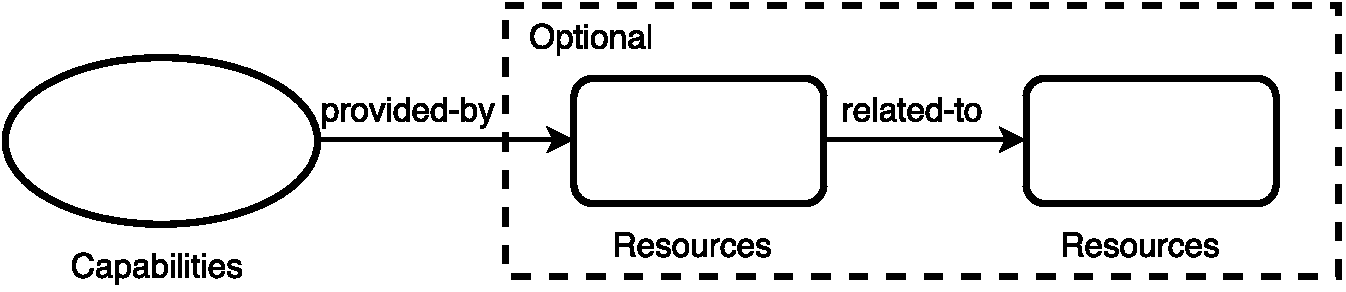
\includegraphics[width=\textwidth,angle=0]{capabilitiesResources.pdf}
	\caption{Capabilities Resources Relationship}
	\label{fig:capabilitiesresources}
\end{figure}

Each \textit{intention} can require certain \textit{capabilities} which are provided by \textit{organizational resources}. 
As a result each informal process model is a strategy and will have cross-functional capabilities, resources (which will be created out of capabilities), a goal that the specific strategy.

For cost calculations of instance descriptors:

For every unspecified instance cost, we go recursively to the lower levels. Assuming that we start our calculation from intentions, with an instance descriptor with id a. We start iterating through every contained achieving strategy, and for each achieving strategy, we iterate through their instance descriptors. In case the parent instance id of an instance descriptor contained in an achieving strategy „a“, then this is relevant for us. In case it’s already specified we directly add it to our summation and proceed with the next instance descriptor and then with the next achieving strategy. In case the cost of an instance descriptor of a strategy has not been specified, we specify it by calculating the cost of instance descriptors of associated informal process definitions. For informal process definitions, we use the cost resource definitions. But you can assume that in each instance descriptor of informal process definition, we already have the cost specified. So this is the end point of the recursion.

%%%%%%%%%%%%%%%%%%%%%%%%%%%%%%%%%%%%%%%%%%%%%%%%%%%%%%%%%%%%%%%%%%%%%%%%%
\subsection{Acquirable Entity Types}
\label{sec:acquirableentities}
%%%%%%%%%%%%%%%%%%%%%%%%%%%%%%%%%%%%%%%%%%%%%%%%%%%%%%%%%%%%%%%%%%%%%%%%%
Final state of the model instance is saved\ref{fig:acquirableentities}.

\begin{figure}
	\centering
	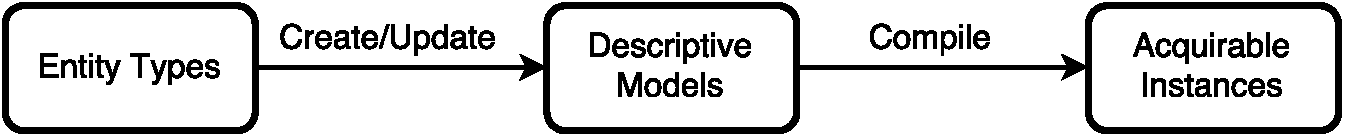
\includegraphics[width=\textwidth,angle=0]{AcquirableEntities.pdf}
	\caption{Acquirable Instances}
	\label{fig:acquirableentities}
\end{figure}



